\documentclass[final]{beamer}

% ====================
% Packages
% ====================

\usepackage[T1]{fontenc}
\usepackage{lmodern}
\usepackage[size=custom,width=84,height=119,scale=1.0]{beamerposter}
\usetheme{gemini}
\usecolortheme{gemini}
\usepackage{graphicx}
\usepackage{booktabs}
\usepackage{tikz}
\usepackage{pgfplots}
\pgfplotsset{compat=1.14}
\usepackage{anyfontsize}
\usepackage[version=4]{mhchem}
\usepackage{siunitx}
\DeclareSIUnit\bar{bar}
\usepackage{overpic}
\usepackage{wasysym}

\usepackage{epstopdf}
\epstopdfDeclareGraphicsRule{.tif}{png}{.png}{convert #1 \OutputFile}
\AppendGraphicsExtensions{.tif}
 
% ====================
% Lengths
% ====================

% If you have N columns, choose \sepwidth and \colwidth such that
% (N+1)*\sepwidth + N*\colwidth = \paperwidth
\newlength{\sepwidth}
\newlength{\colwidth}
\setlength{\sepwidth}{0.025\paperwidth}
\setlength{\colwidth}{0.3\paperwidth}

\newcommand{\separatorcolumn}{\begin{column}{\sepwidth}\end{column}}

% ====================
% Title
% ====================

\title{How much can BCDI contribute to the study of heterogeneous catalysis?}

\author{David Simonne \inst{1, 2, 3}, \and Marie-Ingrid Richard \inst{3, 4}, \and Corentin Chatelier \inst{3, 4}, \and Maxime Dupraz \inst{3, 4}, \and Alina Vlad \inst{1}, \and Benjamin Voisin \inst{1}, \\ \and Yves Garreau \inst{1}, \and Eugene Rabkin \inst{5}, \and Alessandro Coati \inst{1}, \and Andrea Resta \inst{1}}

\institute[shortinst]{\inst{1} Synchrotron SOLEIL - France \samelineand \inst{2} Universite Paris-Saclay - France \samelineand \inst{3} CEA Grenoble - France \samelineand \inst{4} The European Synchrotron - France \samelineand \inst{5} Technion - Israel Institute of Technology - Israel}

% ====================
% Footer (optional)
% ====================

\footercontent{
  \href{https://github.com/DSimonne/PosterCoherence2024}{github.com/DSimonne/PosterCoherence2024}\hfill
  Coherence 2024, MAX IV,  Helsingborg \hfill
  \href{mailto:dsimonne@mit.edu}{dsimonne@mit.edu}}
% (can be left out to remove footer)

% ====================
% Logo (optional)
% ====================

% use this to include logos on the left and/or right side of the header:
% \logoright{\includegraphics[height=5cm]{Figures/Logos/LogoCEA.png}}
% \logoleft{\includegraphics[height=5cm]{Figures/Logos/LogoSaclay.png}}

% ====================
% Body
% ====================

\begin{document}

\begin{frame}[t]
\begin{columns}[t]
\separatorcolumn

\begin{column}{\colwidth}

    \begin{block}{Heterogeneous catalysis}

        \begin{itemize}
        \itemsep 1.5ex
            \item Increases the \textbf{reaction rate}.
            \item Catalyst is in a \textbf{different phase} from the reactants.
            \item Creation of a \textbf{new} reaction path with a \textbf{lower} activation energy.
            \item The \textbf{selectivity} of a specific reaction can also increase.
        \end{itemize}

        \heading{Heterogeneous catalysis is by essence a surface process, in which each reaction step occurs near/on the catalyst surface.}

        \begin{table}[]
        \begin{tabular}{@{}ll@{}}
        \toprule
        Step number & Reaction                                              \\
        \midrule
        1           & \ce{NH3} + \{ \} \textrightarrow \{\ce{NH3}\}       	\\
        2           & \{\ce{NH3}\} \textrightarrow \ce{NH3} + \{ \}       	\\
        3           & \ce{O2} + 2 ( ) \textrightarrow 2 (O)              	\\
        4           & 2 (O) \textrightarrow \ce{O2} + 2 ( ) 				\\
        5           & \{\ce{NH3}\} + 3 (O) \textrightarrow \{N\} + 3 (OH)	\\
        6           & \{N\} + \{N\} \textrightarrow \ce{N2} + 2 \{ \}     	\\
        7           & \{N\} + \{NO\} \textrightarrow \ce{N2O} + 2 \{ \}   	\\
        8           & \{NO\} + ( ) \textrightarrow \{N\} + (O)				\\
        9           & (OH) + (OH) \textrightarrow (O) + ( ) + \ce{H2O}    	\\
        10          & \{N\} + (O) \textrightarrow {NO} + ( ) 				\\
        11          & \ce{H2O} + ( ) + (O) \textrightarrow (OH) + (OH)		\\
        12          & {NO} \textrightarrow NO + \{ \} 							\\
        13          & \ce{N2O} + ( ) \textrightarrow \ce{N2} + (O) 			\\
        \bottomrule
        \end{tabular}
        \caption{Dual sites reaction model for \ce{NH3} oxidation on Pt catalyst \cite{Rebrov2002}.
        \{\} denotes hollow sites, () top and bridge sites on Pt(100).
        %, \ce{NH3} partial pressure: \qtyrange{0.01}{0.12}{\bar}; \ce{O2} partial pressure: \qtyrange{0.10}{0.88}{\bar}; temperature: \qtyrange{125}{375}{\degreeCelsius}; contact time: \qtyrange{0.3}{0.7}{\milli\second}.
        }
        \label{tab:TableReaction}
        \end{table}
    
    \end{block}

    \begin{alertblock}{The example of ammonia oxidation}

    \vspace{-1cm}
               
        \begin{align}
            \label{eq:AmmoniaOxidationNitrogen}
            4 \ce{NH3} + 3 \ce{O2} & \rightarrow 6 \ce{H2O} + 2 \ce{N2} \\
            \label{eq:AmmoniaOxidationNitrousOxide}
            4 \ce{NH3} + 4 \ce{O2} & \rightarrow 6 \ce{H2O} + 2 \ce{N2O} \\
            \label{eq:AmmoniaOxidationNitricOxide}
            4 \ce{NH3} + 5 \ce{O2} & \rightarrow 6 \ce{H2O} + 4 \ce{NO}
        \end{align}
       
        \begin{figure}
            \centering
            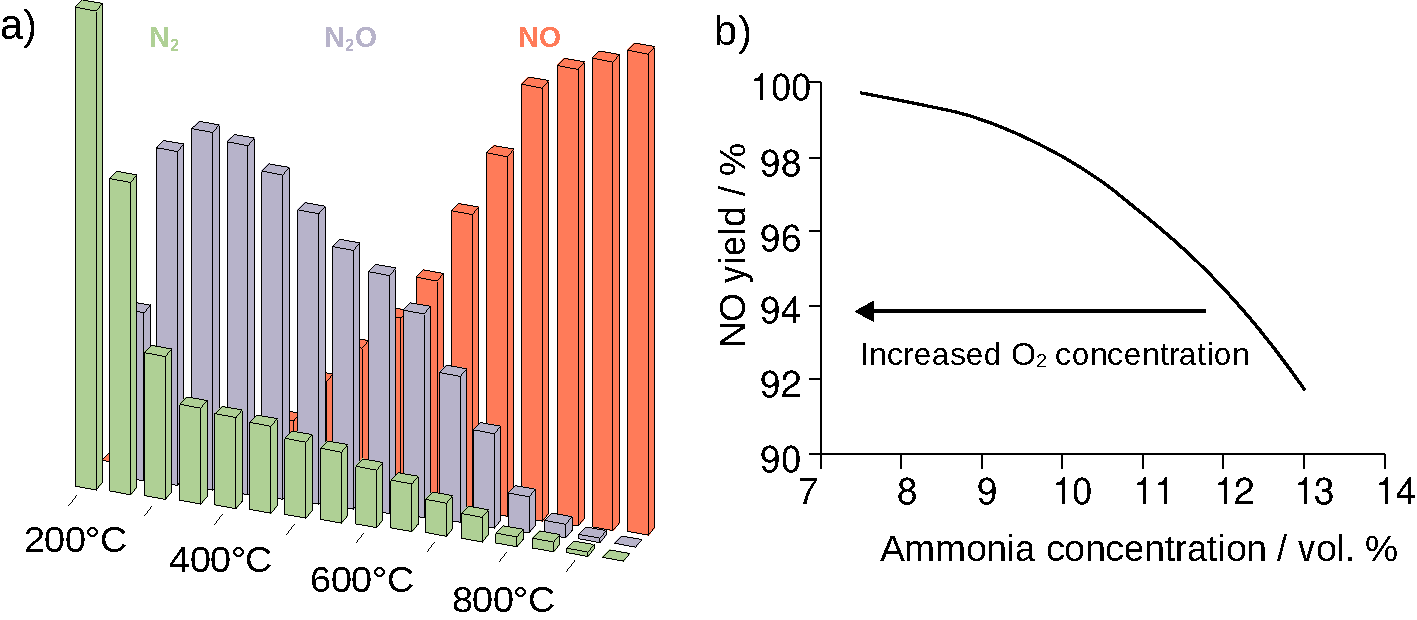
\includegraphics[width=0.95\colwidth]{Figures/UmicoreSlides.pdf}
            \caption{Only at high temperature (a), high \ce{O_2}/\ce{NH_3} ratios (b), and over catalysers, is the production of \ce{NO} favoured\cite{Hatscher2008}.}
            \label{fig:AmOxHatscher}
        \end{figure}
            
        \heading{The Ostwald process relies on the production of \ce{NO} \textit{via} ammonia oxidation (first step) to produce nitric acid (second step).}

        \vspace{1cm}

        \begin{figure}
            \centering
            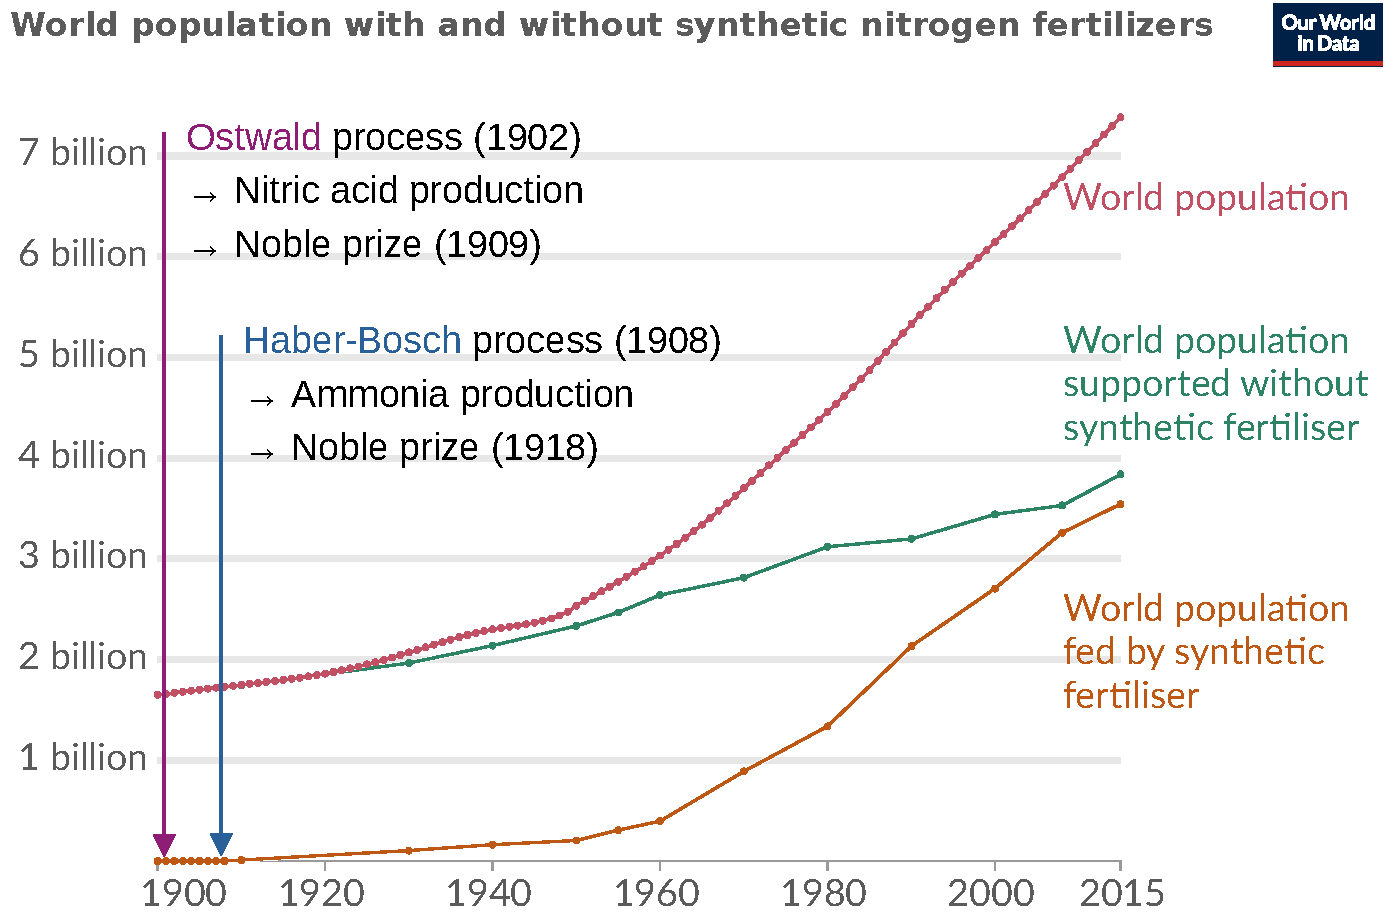
\includegraphics[width=0.95\colwidth]{Figures/WorldPopAmmonia.pdf}
            \caption{The production of \textbf{nitrogen fertilisers} from nitric acid is at the  origin of the \textbf{selective} catalytic ammonia oxidation \cite{Erisman2008}.}
        \end{figure}
                
    \end{alertblock}

    \begin{block}{The material and pressure gap}

        \textit{"A long standing conundrum in the catalysis community emerged at the interface between surface science and heterogeneous catalysis, better known as the pressure and material gap."}
        
        \textbf{Nature Catalysis editorial, 2018.}
        
        \vspace{1cm}

        \begin{table}[!htb]
            \centering
            \begin{tabular}{l|l|l|l}
            \toprule
                        & Pressure    & Material                         &     Temperature \\
            \midrule
            Industry   & \qtyrange{1}{12}{\bar} & Knitted gauzes wires   & \qtyrange{750}{900}{\degreeCelsius} \\
                       &              & (diameter \qty{\approx 80}{\um}) & \\
            \midrule
            Literature & UHV, mbar    & Single crystals                  & \qtyrange{25}{900}{\degreeCelsius} \\
            \midrule
            This study & Near ambient & Single crystals                  & \qtyrange{25}{600}{\degreeCelsius} \\
                       & pressure (\qty{0.5}{\bar})  & and nanoparticles & \\
            \bottomrule
            \end{tabular}
            \caption{
                Reproducing \textbf{relevant industrial conditions} relies on the probe, the technique, and the design of reactor cells at synchrotrons.
            }
            \label{tab:Gap}
        \end{table}

    \end{block}

\end{column}

%%%%%%%%%%%%%%%%%%%%%%%%%%%%%%%%%%%%%%%%%%%%%%%%%%%%%%%%%%%%%%%%%%%%%
\separatorcolumn

\begin{column}{\colwidth}

    \begin{block}{Observing chemical reactions indirectly}

        \begin{itemize}
            \itemsep 1.5ex
            \item Molecular/atomic adsorption can lead to \textbf{surface relaxation}, \textbf{roughness}, and \textbf{surface reconstruction} phenomena.
            \item The \textbf{electronic environment} of surface atoms can be impacted by the adsorption of reacting species.
        \end{itemize}
        
        % \begin{figure}
        %     \centering % , trim={0 8cm 0 0}, clip
        %     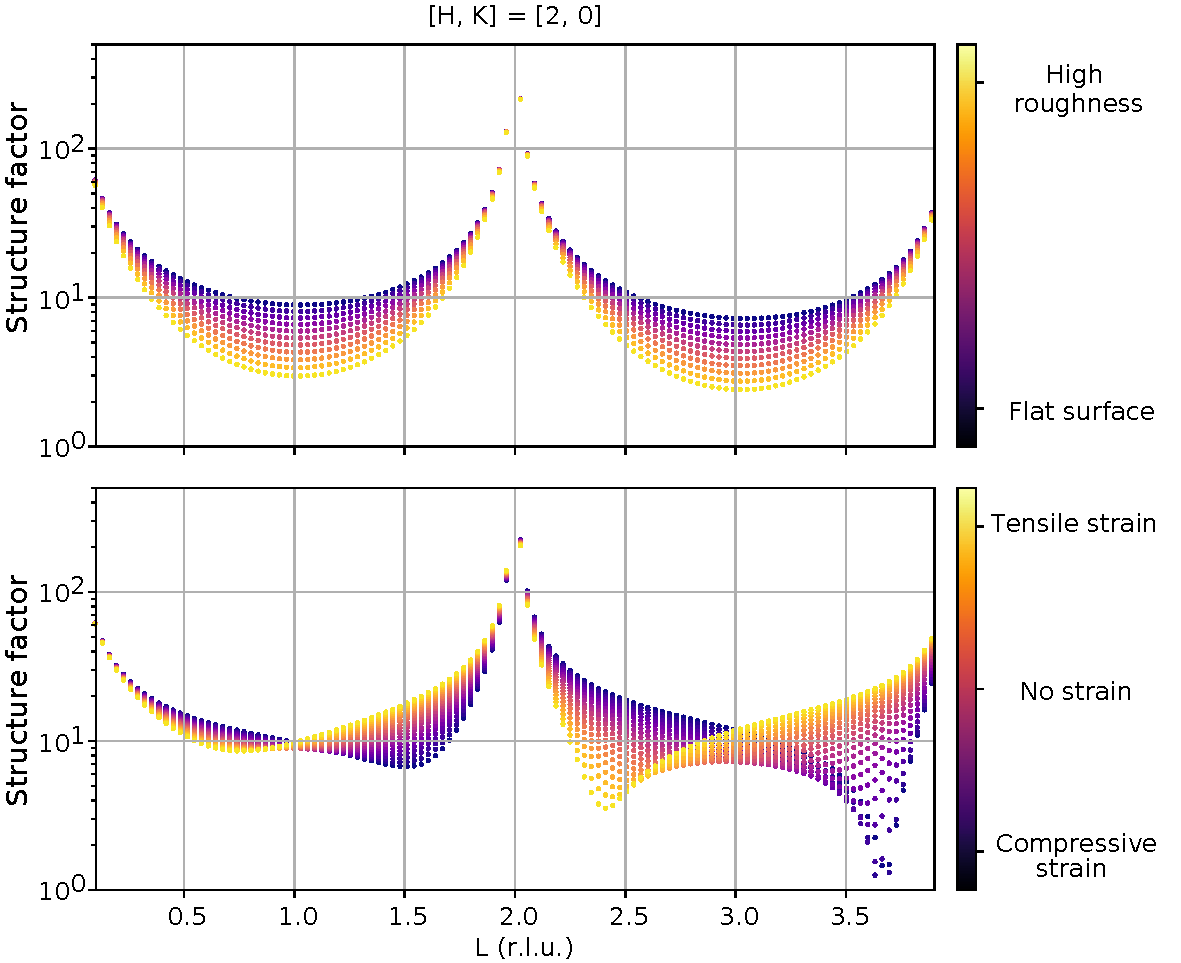
\includegraphics[width=0.95\colwidth]{Figures/relax_rough_ctr_slides.pdf}
        %     \caption{Simulated intensity of Pt(100) crystal truncation rod.}
        %     \label{fig:CTRSimuRelax}
        % \end{figure}
        
    \end{block}

    \begin{block}{BCDI is sensitive to structural changes}

        Obtain (i) the sample Bragg electronic density $\rho(\vec{r})$, and (ii) a \textbf{projection} of the \textbf{displacement field $\vec{u}(\vec{r})$} on the \textbf{scattering vector} $\vec{G}_{hkl}$.

        % Complex object after data reduction: $\rho(\vec{r})e^{i\vec{G}_{hkl}.\vec{u}(\vec{r})}$

        \begin{itemize}
            \itemsep 1.5ex
            \item Sample morphology reconstructed from BCDI measurement.
            \item Full \textbf{displacement field} and associated \textbf{strain tensor}.
            \item Few seconds measurement with nanometer resolution.
        \end{itemize}
    
    \end{block}
    
    \begin{exampleblock}{Pt particles for \textit{in-situ} BCDI}

        \begin{itemize}
            \itemsep 1.5ex
            \item Particles fixed on substrate to avoid movement / sintering.
            \item Large distribution of particle size / morphology.
            \item Epitaxy impacts particle morphology and strain.
        \end{itemize}
    
        \begin{figure}
            % \includegraphics[width=0.3\colwidth]{Figures/SEM/sample00.tif}
            % \includegraphics[width=0.3\colwidth]{Figures/SEM/sample02.tif}
            % \includegraphics[width=0.28\colwidth]{Figures/SEM/sample01.tif}
            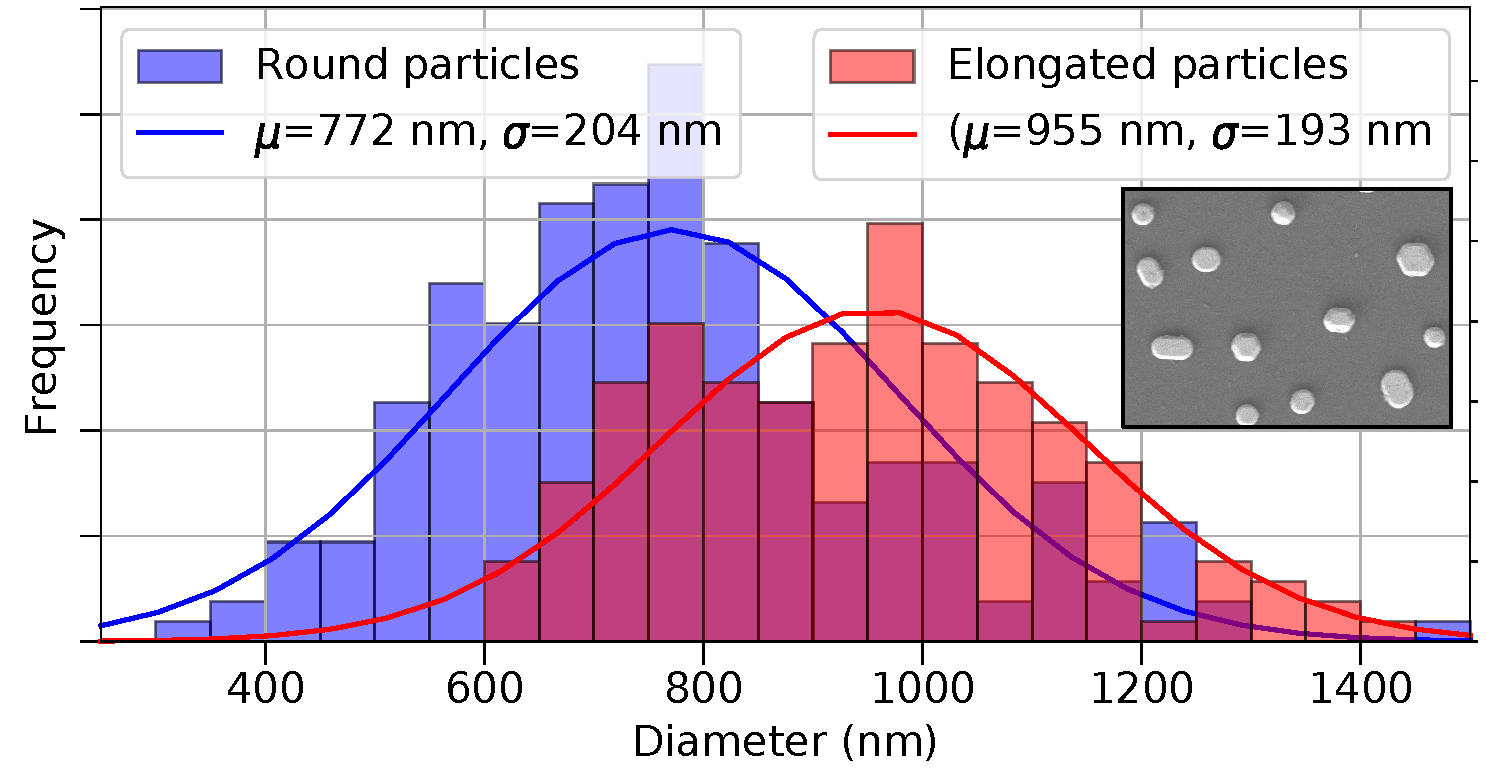
\includegraphics[width=\colwidth]{Figures/SEM/PtSampleClusterDiameterHistLabelled.pdf}
        \end{figure}

        \begin{figure}
            \centering
            \begin{overpic}[width=0.45\linewidth]{Figures/B7.png}
                \put(72, 60){{\diameter \approx\qty{350}{\nm}}}
            \end{overpic}
            \hfill
            \begin{overpic}[width=0.45\linewidth]{Figures/D6.png}
                \put(-7, 60){{\diameter \approx\qty{800}{\nm}}}
            \end{overpic}
            \caption{Top: Histogram of particle size distribution from Scanning Electron Microscopy (SEM). Bottom: BCDI reconstructions.}
        \end{figure}

    \end{exampleblock}
    
    \begin{exampleblock}{Of the importance of particle morphology}

        \begin{figure}
            \centering
            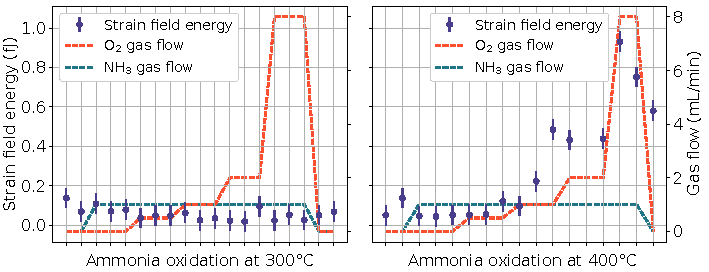
\includegraphics[width=0.95\colwidth]{Figures/SFE.pdf}
            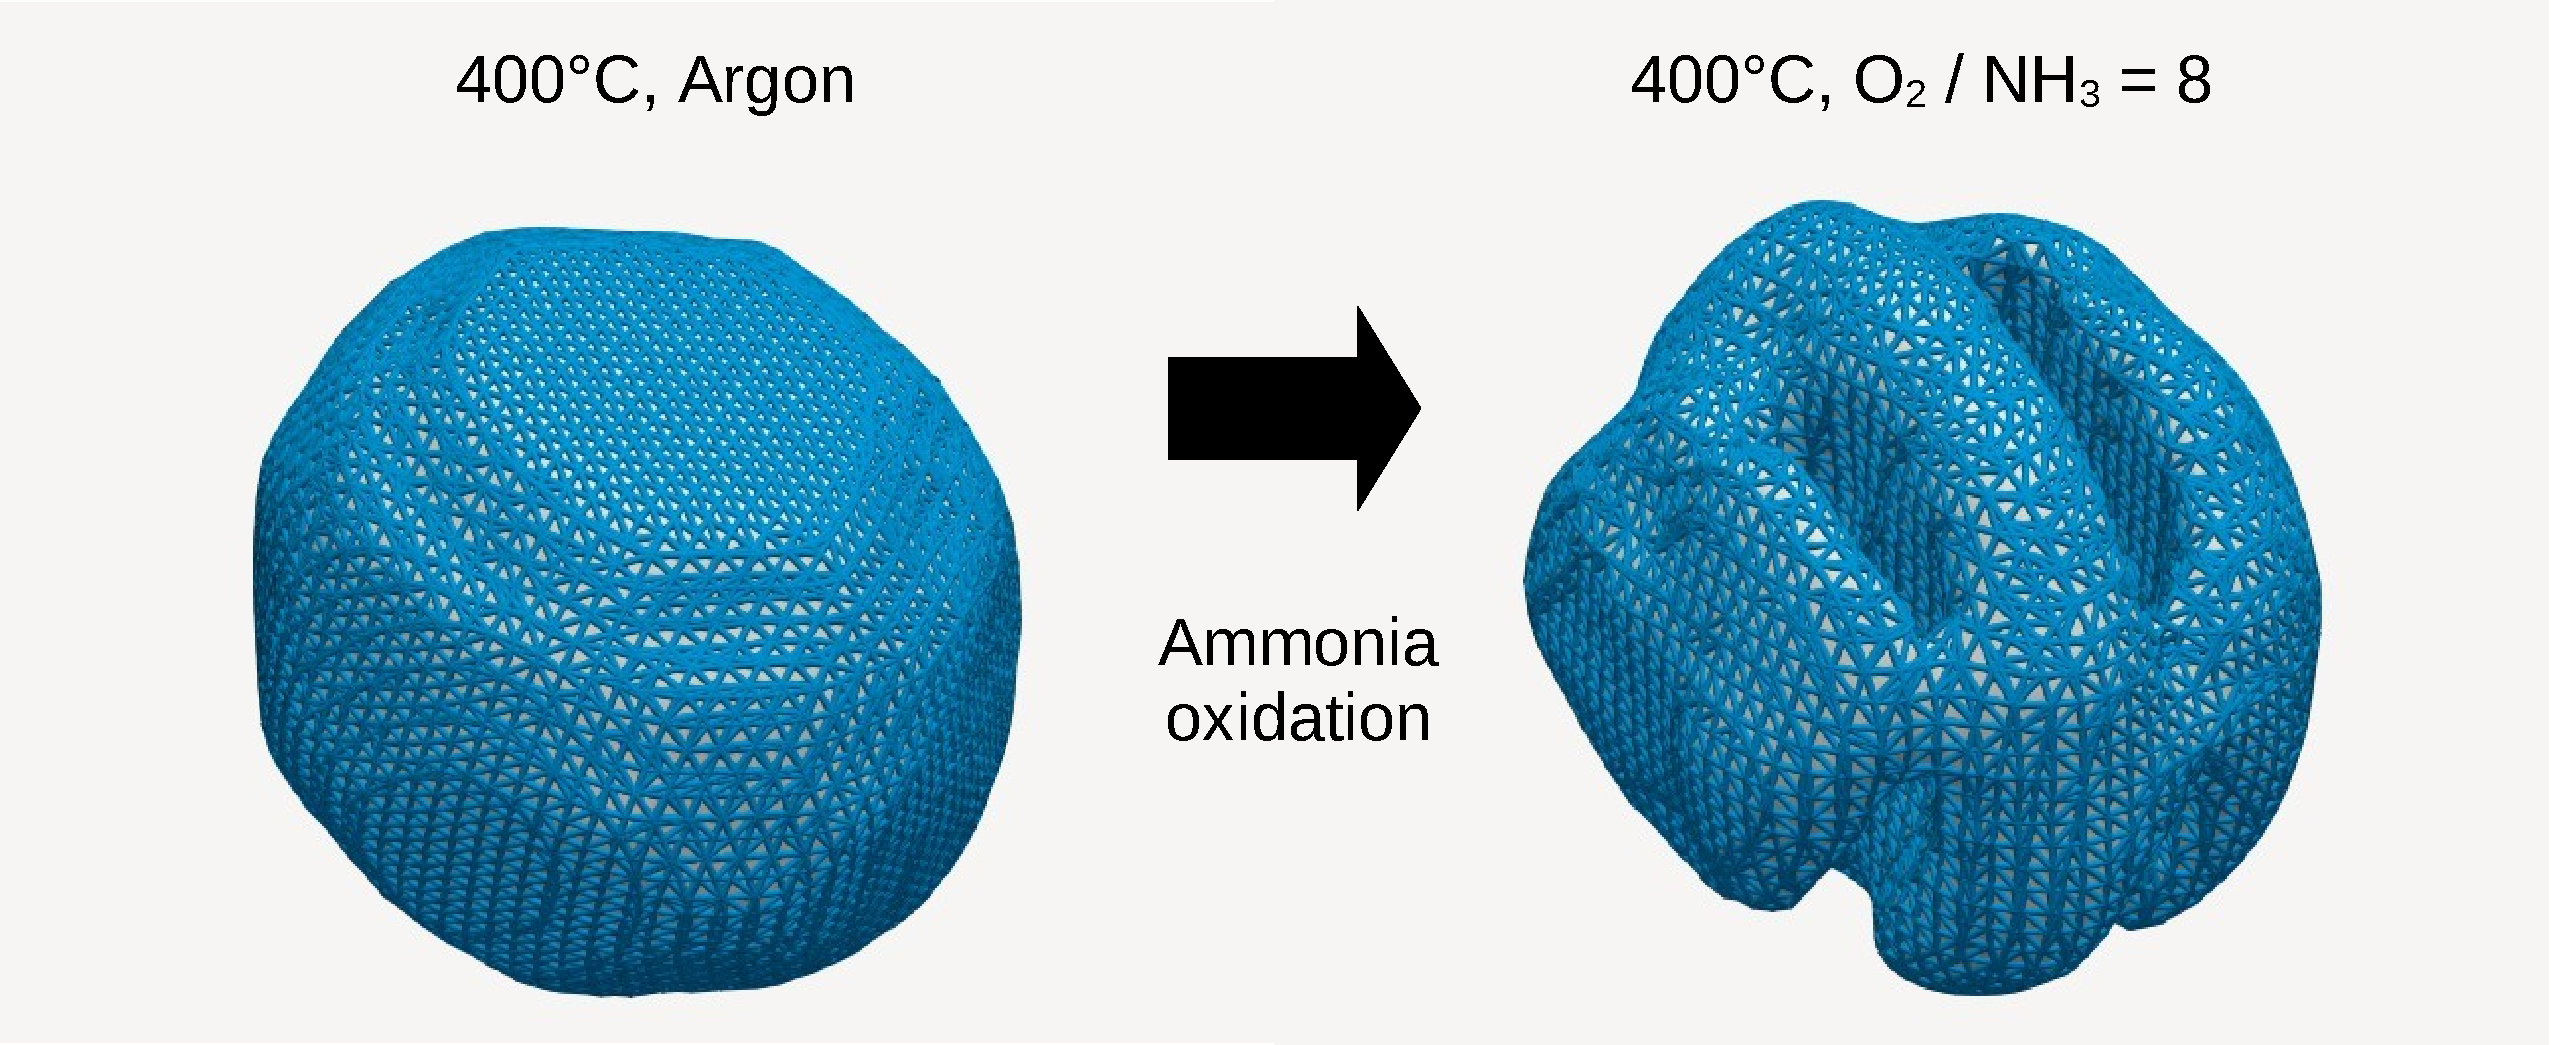
\includegraphics[width=0.95\colwidth]{Figures/B7BeforeAndAfter.pdf}
            \caption{\textit{In-situ} round particle morphology evolution at \qty{400}{\degreeCelsius}.}
            \label{fig:SFE}
        \end{figure}

        \begin{itemize}
            \itemsep 1.5ex
            \item Different evolution for particles of \textbf{different size, morphology (facets), and initial strain state}.
            \item Structural changes at \qty{400}{\degreeCelsius} above \ce{O2} / \ce{NH3} : 1 on round particle, conditions favouring \ce{NO}, defects appear.
            \item Ammonia adsorption poisoning on elongated particle.
        \end{itemize}
        
    \end{exampleblock}
    
    \begin{block}{BCDI offers a limited picture...}
        \begin{itemize}
            \itemsep 1.5ex
            \item Sample size from \qtyrange{100}{1000}{\nm}.
            \item \textbf{Single} measurement process \rightarrow far from collective behaviour.
            \item \textbf{Anisotropic} spatial resolution, \textbf{sample specific}.
            \item Difficult to observe the formation of \textbf{active surface phases}.
        \end{itemize}

        \heading{How to correlate strain changes to facet specific absorption / adsorption phenomena?}
        
    \end{block}
\end{column}

%%%%%%%%%%%%%%%%%%%%%%%%%%%%%%%%%%%%%%%%%%%%%%%%%%%%%%%%%%%%%%%%%%%%%
\separatorcolumn

\begin{column}{\colwidth}

    \begin{exampleblock}{... completed by other techniques}

        \heading{Surface X-ray diffraction}

        \begin{figure}
            \centering
            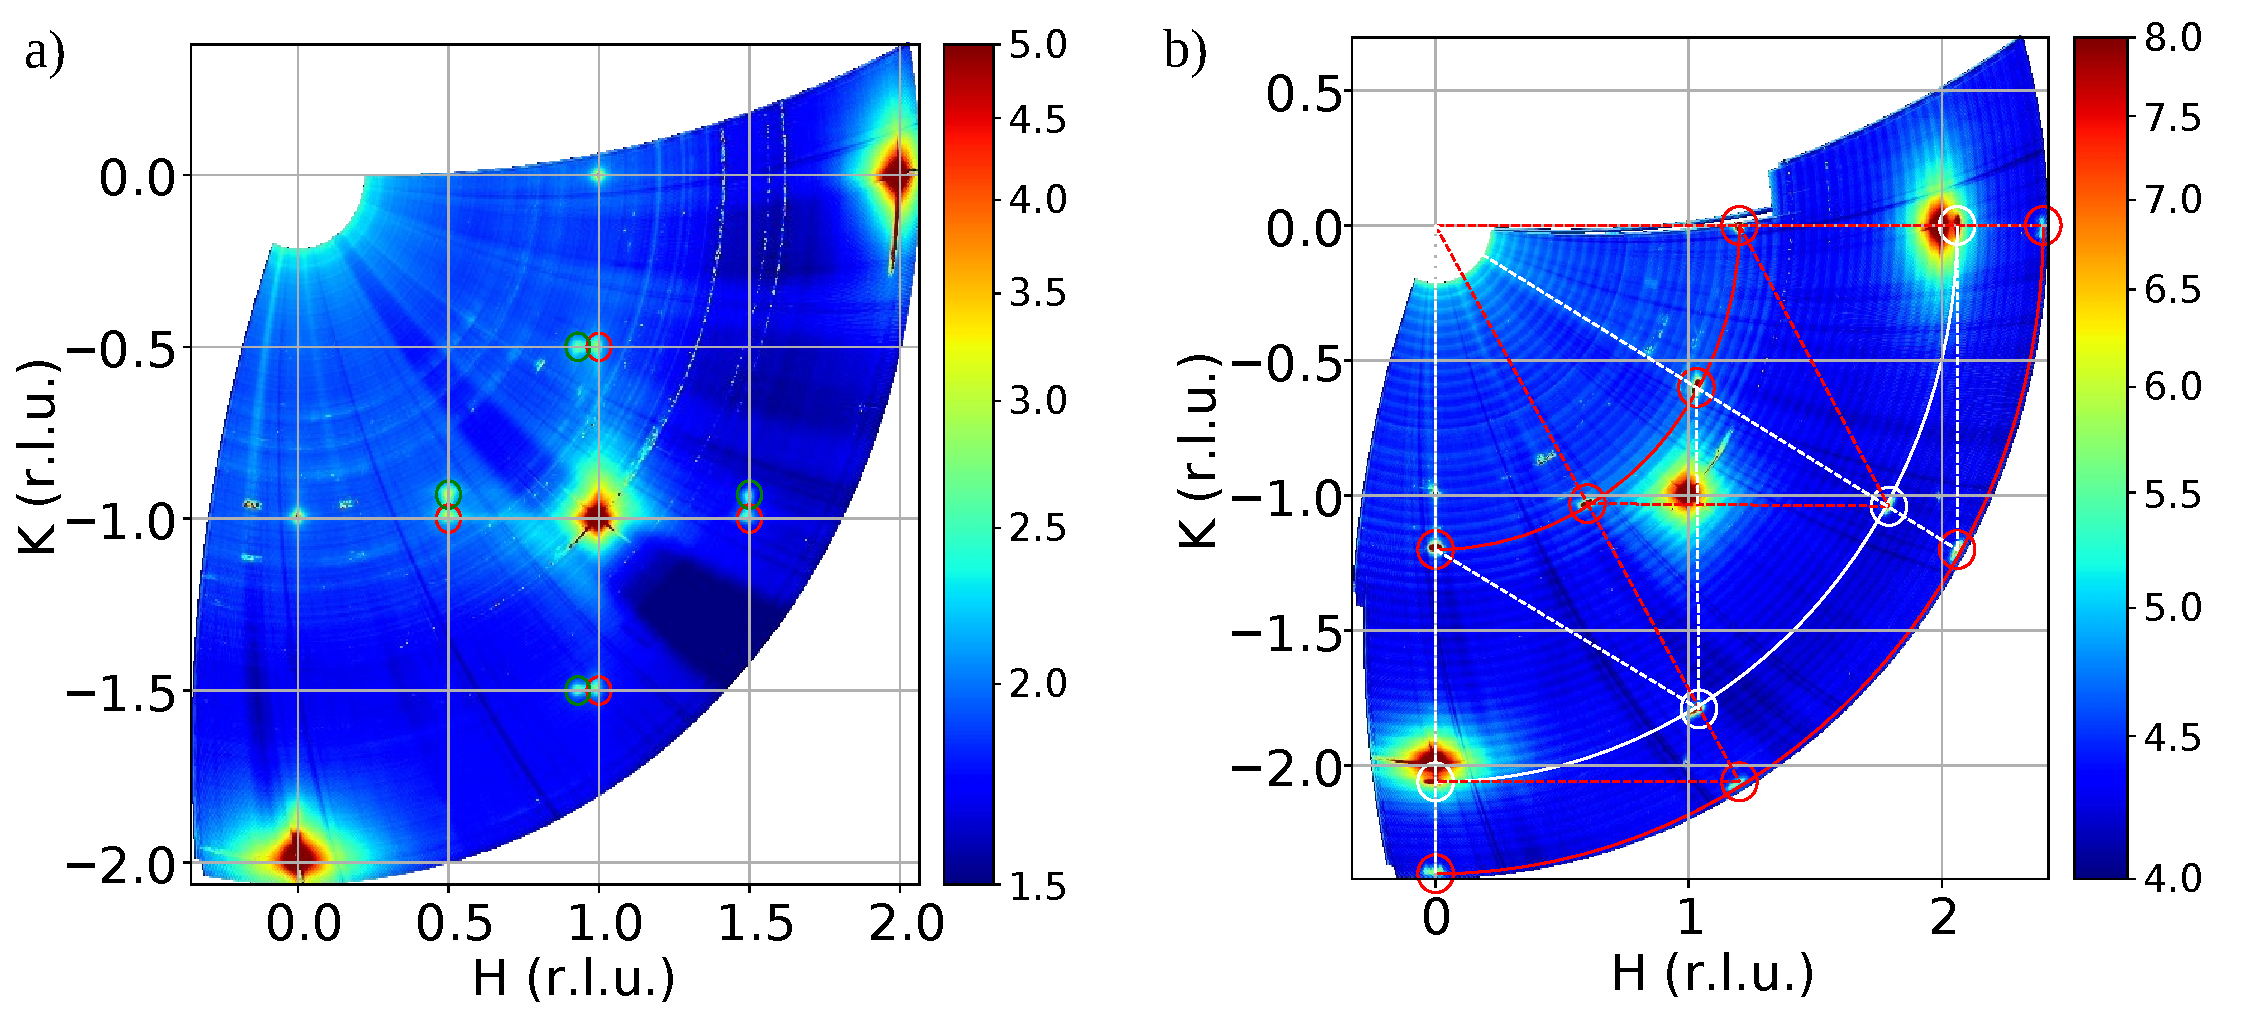
\includegraphics[width=0.95\colwidth]{Figures/Maps.pdf}
            \caption{Pt(100) reciprocal space in-plane maps \textrightarrow \textbf{Presence of active surface phases such as surface oxides (a) and surface reconstructions (b) during ammonia oxidation at \qty{450}{\degreeCelsius}}.}
            \label{fig:Pt100SurfRec}
        \end{figure}

        \begin{figure}
            \centering
            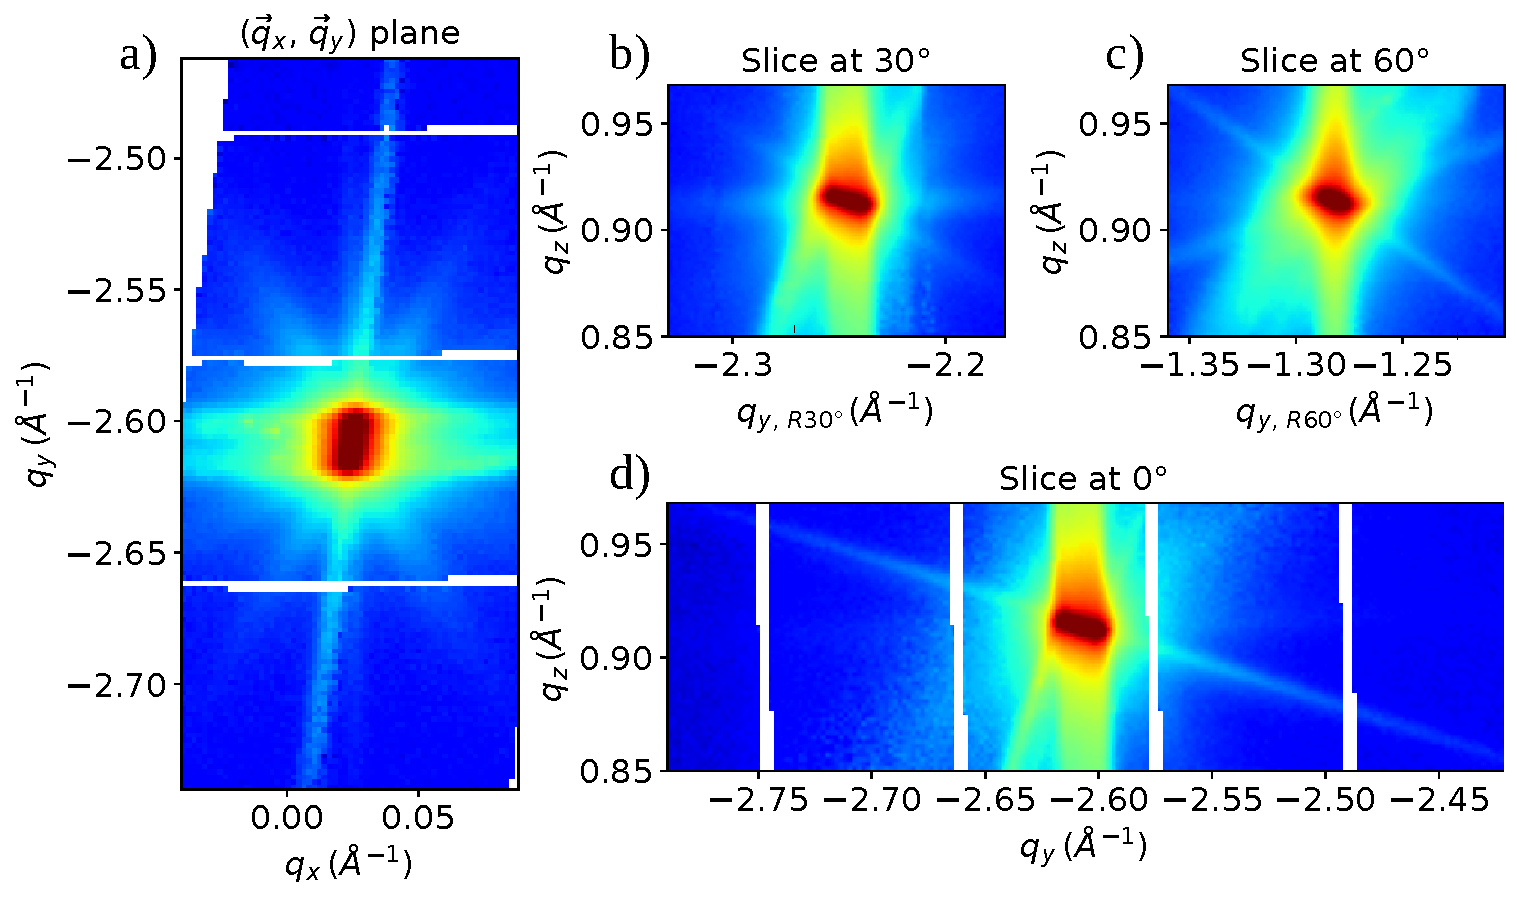
\includegraphics[page=1, width=0.95\colwidth]{Figures/FacetsTogether.pdf}
            \caption{Crystal truncation rods from facets on Pt particles \rightarrow \textbf{Collective behaviour such as particle reshaping}.}
        \end{figure}

        \begin{figure}
            \centering
            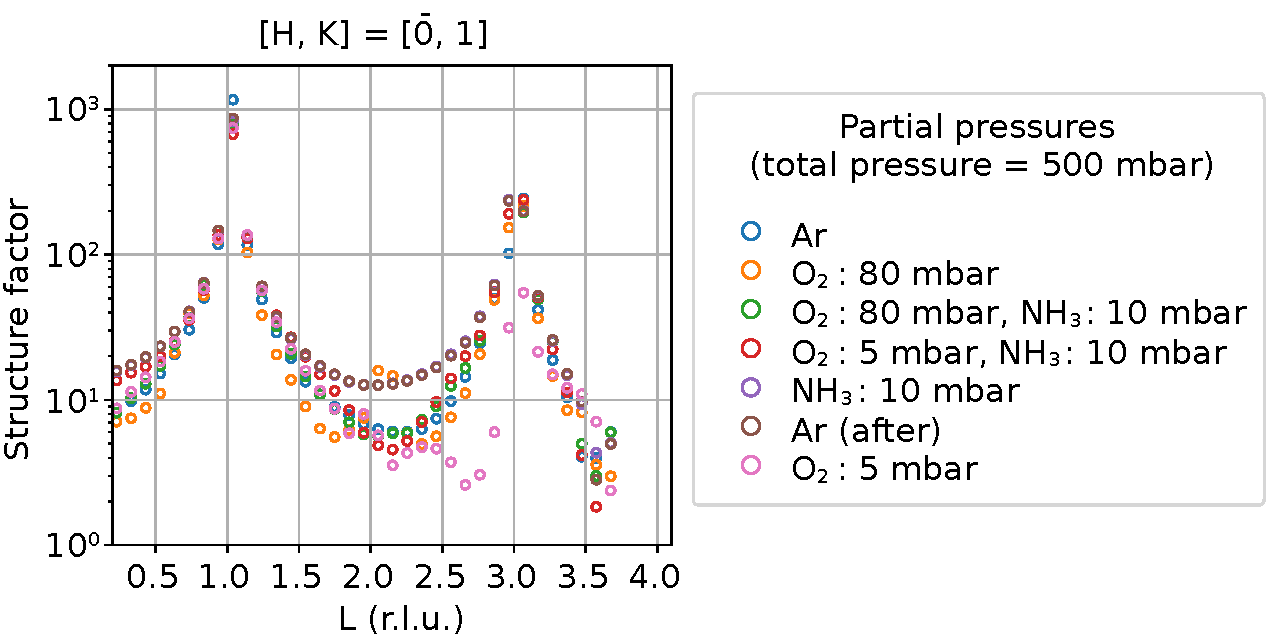
\includegraphics[width=0.95\colwidth]{Figures/CTR.pdf}
            \caption{Pt(100) crystal truncation rods \rightarrow \textbf{Surface roughness and relaxation effects}.}
        \end{figure}

        \heading{X-ray photoelectron spectroscopy}

        \begin{figure}
            \centering
            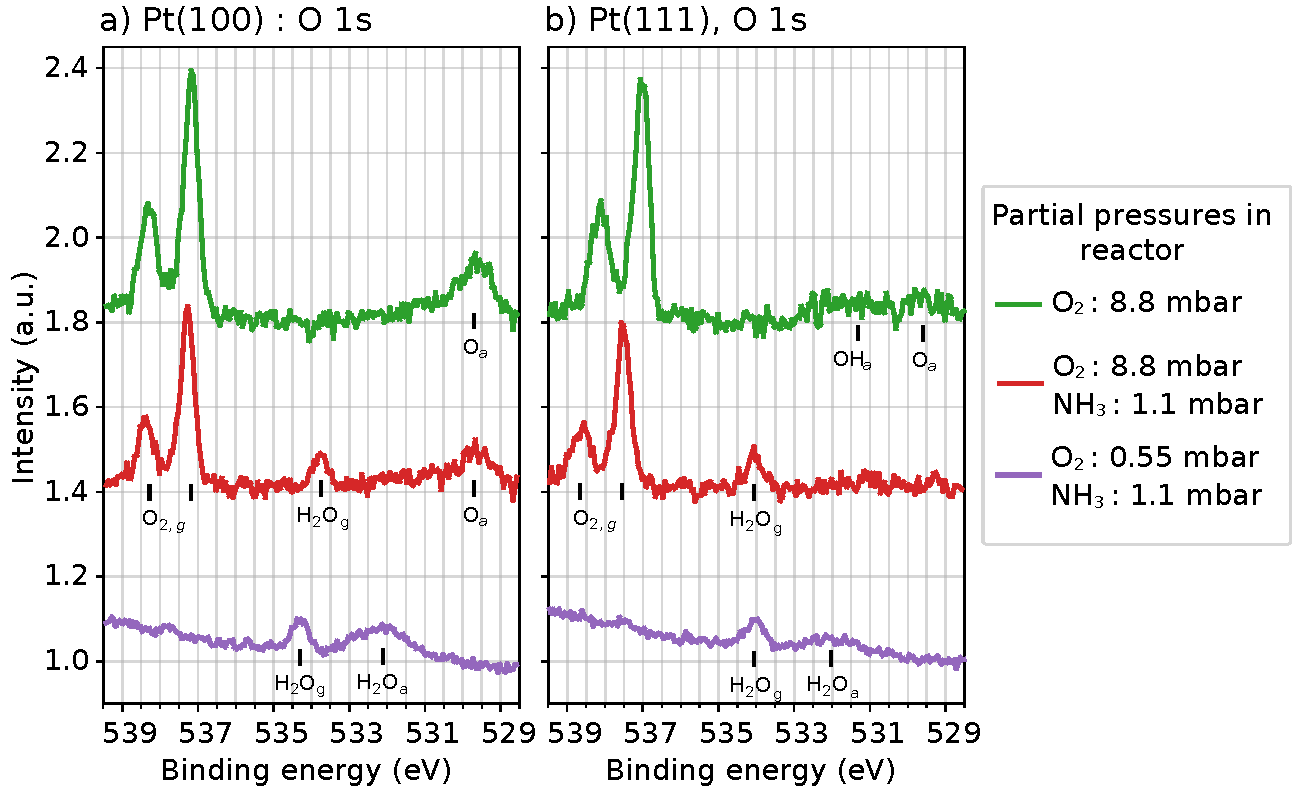
\includegraphics[width=0.9\colwidth]{Figures/O1sSlidesBis.pdf}
            \caption{XPS spectra collected at the O 1s (a) and N1 s (b) levels under different atmospheres at \qty{450}{\degreeCelsius} \rightarrow \textbf{Difference in quantity / nature of adsorbed active surface species.}}
            \label{fig:XPS}
        \end{figure}

    \end{exampleblock}

    \vspace{-0.5cm}

    \begin{block}{References}

        \nocite{*}
        \footnotesize{\bibliographystyle{abbrv}\bibliography{references}}

    \end{block}

    \begin{block}{Acknowledgements}
    
        \centering

        \footnotesize{This project received funding from the European Research Council (ERC) under the European Union’s Horizon 2020 research and innovation program (grant agreement No. 818823.)}
                
        \begin{figure}
            \centering
            
\includegraphics[height=2.15cm]{Figures/Logos/LogoSoleil.png}
            
\includegraphics[height=2.15cm]{Figures/Logos/CEA.png}
            
\includegraphics[height=2.15cm]{Figures/Logos/ParisSaclayBlanc.png}
            
\includegraphics[height=2.15cm]{Figures/Logos/logocarine.png}
            
\includegraphics[height=2.15cm]{Figures/Logos/logosixs.jpg}
        \end{figure}
        
    \end{block}
    
\end{column}

\separatorcolumn
\end{columns}
\end{frame}

\end{document}
